\chapter{Methods}

\section{Dataset}

This study used a retrospective dataset of abdominal ultrasound examinations from pancreas transplant recipients at Hospital Cl\'{i}nic de Barcelona, collected between October 2016 and January 2020. The cohort comprised 56 patients who underwent a total of 138 imaging studies as part of routine post-transplant surveillance. Each study corresponds to a single ultrasound examination session, identified by a unique study identifier of the form \texttt{XX\_YY}, where \texttt{XX} denotes the patient and \texttt{YY} the visit number for that patient. The number of studies per patient ranged from 1 to 7, with a mean of 2.5 studies per patient.

Imaging was performed using a Siemens Acuson S3000 ultrasound system. Each examination included three imaging modalities: conventional grayscale B-mode ultrasound, Acoustic Radiation Force Impulse (ARFI) elastography, and dynamic contrast-enhanced ultrasound (DCE-US). The present work focuses exclusively on the grayscale B-mode images for radiomics analysis, while ARFI and DCE-US measurements from the clinical records are used for comparison with previously published results.

Each study was classified as either ``rejection'' or ``no rejection'' based on the clinical variable \texttt{motivo} recorded in the patient database. This variable encodes the clinical reason for each examination and was mapped to a binary outcome: studies where the recorded reason indicated biopsy-confirmed or clinically suspected rejection were labelled as rejection, and all others as no rejection.

An important characteristic of this dataset is its repeated-measures structure: individual patients contribute multiple studies across different time points, and the same patient may have studies in both outcome classes at different visits. A total of 14 patients had studies in both the rejection and no-rejection groups. This structure violates the assumption of independence between samples that underlies standard statistical tests and cross-validation procedures, a limitation that is addressed explicitly in the experimental design (see Section~\ref{sec:statistical_analysis}).

One study (47\_01) was excluded from all analyses because the hospital confirmed that the images were never recovered from the imaging system and could not be made available. This study was a rejection case, reducing the cohort to 55 patients contributing 137 studies. Of these, 98 were classified as no rejection and 39 as rejection, yielding a class imbalance ratio of approximately 71:29. All 137 studies had both radiomics features and matching clinical records, forming the merged dataset used for all subsequent analyses.

\begin{table}[ht]
\centering
\caption{Summary of the dataset used in this study.}
\label{tab:dataset_summary}
\begin{tabular}{lr}
\toprule
Characteristic & Value \\
\midrule
Number of patients & 56 \\
Total imaging studies & 138 \\
Studies with radiomics features & 137 \\
Studies in merged dataset & 137 \\
No rejection studies & 98 \\
Rejection studies & 39 \\
Class ratio (no rejection : rejection) & 71:29 \\
Studies per patient (mean $\pm$ range) & 2.5 (1--7) \\
Patients with both outcomes & 14 \\
Collection period & Oct 2016 -- Jan 2020 \\
Imaging system & Siemens Acuson S3000 \\
\bottomrule
\end{tabular}
\end{table}

Figure~\ref{fig:patient_flow} summarises the study selection process and the final class distribution used in all analyses.

\begin{figure}[ht]
\centering
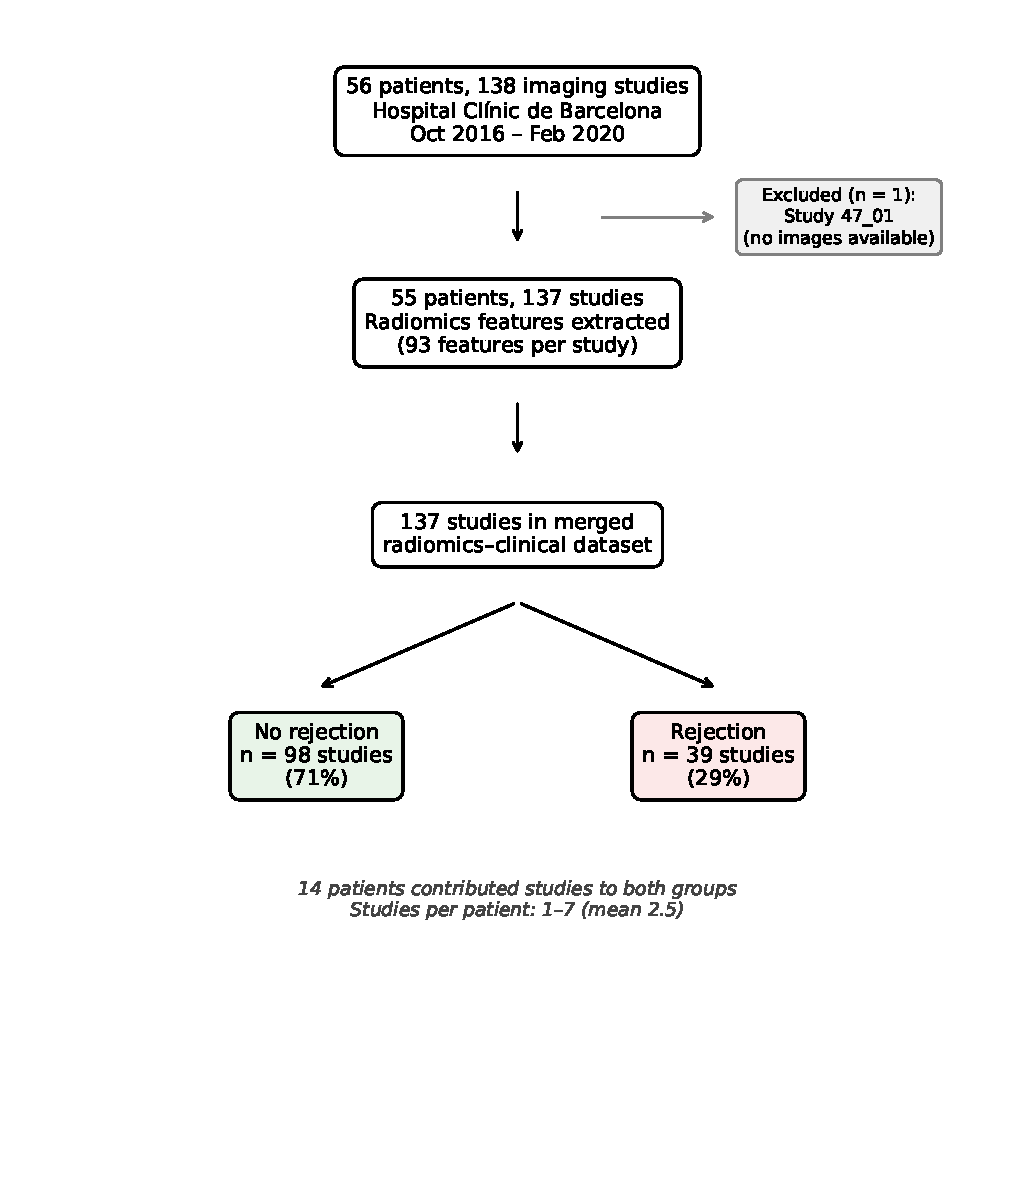
\includegraphics[width=0.65\textwidth]{Figures/patient_flow.pdf}
\caption{Patient flow diagram showing study selection and outcome classification. Of the 138 imaging studies from 56 patients, one was excluded due to missing images. The remaining 137 studies were merged with clinical records and classified as rejection ($n = 39$) or no rejection ($n = 98$).}
\label{fig:patient_flow}
\end{figure}


\section{Image Preprocessing}
\label{sec:preprocessing}

The raw DICOM images contained clinician-drawn white contour annotations delineating the region of interest (ROI) around the pancreas graft. These annotations, while essential for identifying the tissue region, would introduce high-intensity artifacts into texture-based radiomics features if not removed prior to feature extraction. The preprocessing pipeline was therefore designed to extract the tissue region defined by the annotation while excluding the contour line itself.

The preprocessing consisted of the following steps:

\begin{enumerate}
\item \textbf{DICOM loading and white pixel detection.} Each DICOM file was loaded as an RGB image. Pixels belonging to the clinician-drawn contour were identified using an intensity threshold: pixels with values exceeding 250 on all three colour channels were classified as contour pixels.

\item \textbf{Connected component filtering.} Multiple white regions may exist in an ultrasound image due to interface elements, scale bars, or other annotations. To isolate the clinician-drawn contour, only the largest connected component of detected white pixels was retained.

\item \textbf{Morphological closing.} A morphological closing operation was applied to bridge small gaps in the contour line, ensuring a continuous closed boundary. This step used a circular structuring element.

\item \textbf{Contour filling and subtraction.} The closed contour was filled to produce a solid binary mask covering the entire annotated region. The original contour pixels were then subtracted from this filled mask, yielding a mask that includes only the tissue interior without the bright annotation border.

\item \textbf{Grayscale conversion.} The RGB image was converted to grayscale for radiomics feature extraction.

\item \textbf{Mask erosion.} The binary mask was eroded using a $3 \times 3$ square kernel with one iteration to further reduce boundary artifacts from partial contour pixels or edge effects at the tissue--background interface.
\end{enumerate}

The final outputs for each study were a binary mask image and a segmented grayscale image (the original image multiplied by the mask). These were stored in the preprocessed dataset directory and used as inputs for radiomics feature extraction.

Two studies required special handling. Study 03\_01 exhibited a dimension mismatch between the mask and image arrays, which was resolved by transposing the mask to match the image orientation. Study 43\_01 had an incompletely closed clinician contour, causing the fill operation to collapse. This was addressed by applying a substantially larger morphological closing kernel to force closure of the contour before filling.

Figure~\ref{fig:preprocessing} illustrates the preprocessing pipeline for an example study. Panel~(a) shows the original grayscale ultrasound image with the clinician-drawn white contour delineating the pancreas graft. Panel~(b) shows the binary mask obtained after white pixel detection, connected component filtering, morphological closing, contour filling, and contour subtraction. Panel~(c) shows the mask after erosion, and panel~(d) shows the final segmented tissue region used as input for radiomics feature extraction.

\begin{figure}[ht]
\centering
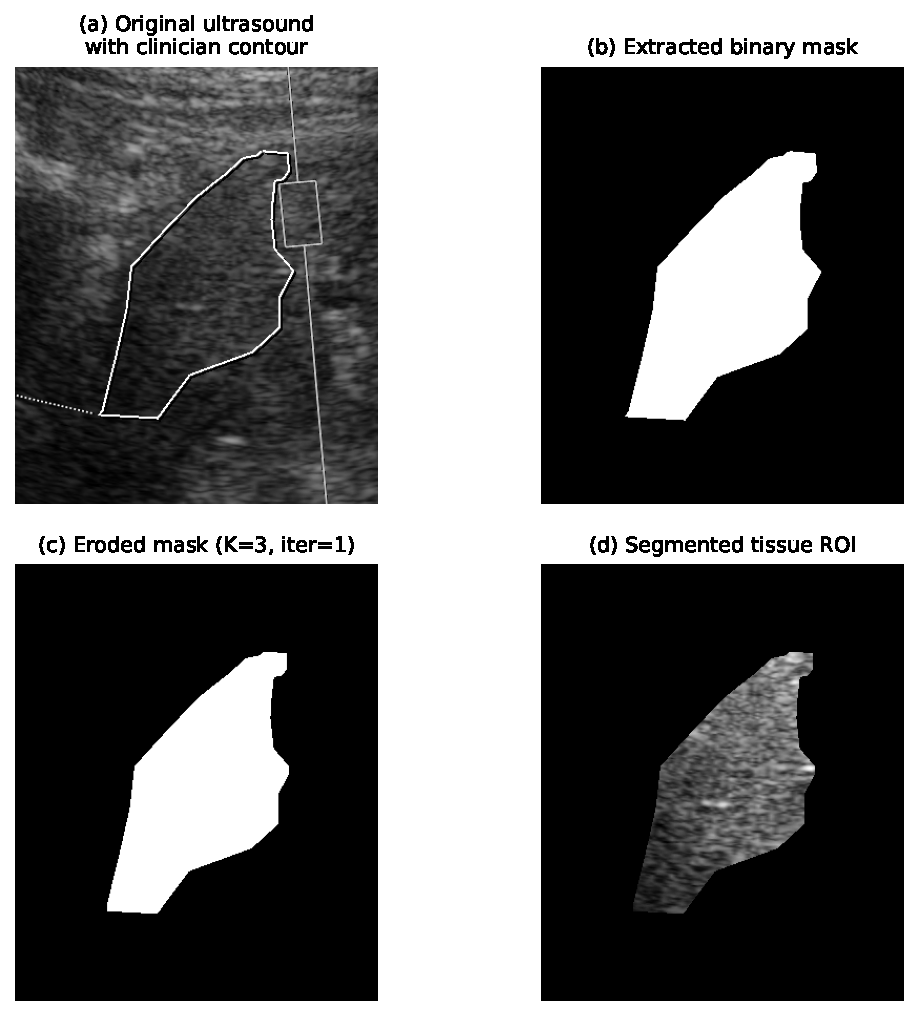
\includegraphics[width=0.85\textwidth]{Figures/preprocessing_pipeline.pdf}
\caption{Preprocessing pipeline illustrated on study 10\_01. (a)~Original B-mode ultrasound with clinician-drawn contour annotation. (b)~Binary mask after contour detection, filling, and subtraction. (c)~Eroded mask ($3 \times 3$ kernel, 1 iteration). (d)~Final segmented tissue region of interest.}
\label{fig:preprocessing}
\end{figure}


\section{Radiomics Feature Extraction}
\label{sec:feature_extraction}

Radiomics features were extracted from the preprocessed grayscale images using PyRadiomics (version 3.0) \cite{vanGriethuysen2017}, an open-source Python library that implements the feature definitions standardised by the Image Biomarker Standardisation Initiative (IBSI) \cite{zwanenburg2020}.

Feature extraction was configured with the following settings: images were processed in two-dimensional mode (\texttt{force2D = True}), as each study consisted of a single ultrasound slice rather than a volumetric scan. Pixel intensities were discretised using a fixed bin width of 25 grey levels (\texttt{binWidth = 25}), and images were cast to 16-bit signed integers prior to extraction. Shape-based features were disabled, as ultrasound ROI shapes are determined by the clinician's annotation rather than by the underlying tissue morphology.

A total of 93 features were extracted per study across six texture and intensity feature classes, summarised in Table~\ref{tab:feature_classes}.

\begin{table}[ht]
\centering
\caption{Radiomics feature classes extracted using PyRadiomics. Shape features were excluded.}
\label{tab:feature_classes}
\begin{tabular}{llr}
\toprule
Feature class & Description & Count \\
\midrule
First Order & Intensity histogram statistics & 18 \\
GLCM & Grey-level co-occurrence matrix & 24 \\
GLRLM & Grey-level run-length matrix & 16 \\
GLSZM & Grey-level size-zone matrix & 16 \\
GLDM & Grey-level dependence matrix & 14 \\
NGTDM & Neighbourhood grey-tone difference matrix & 5 \\
\midrule
\textbf{Total} & & \textbf{93} \\
\bottomrule
\end{tabular}
\end{table}

First-order features describe the distribution of individual pixel intensities within the ROI, capturing properties such as mean, variance, skewness, and entropy. The remaining five classes are texture features that quantify spatial relationships between pixel intensities. GLCM features measure pairwise co-occurrences of grey levels at specified offsets, characterising patterns of local texture. GLRLM features describe runs of consecutive pixels with the same grey level, capturing coarseness and directionality. GLSZM features quantify contiguous zones of uniform intensity regardless of direction. GLDM features measure dependencies between a pixel and its neighbours, and NGTDM features describe how each grey level differs from the average of its neighbourhood.

Feature extraction was applied to all 137 preprocessed studies, producing a feature matrix of 137 rows (studies) and 93 columns (features). No extraction failures occurred. This matrix was merged with the clinical database; all 137 studies had matching clinical records, yielding a complete dataset for downstream analysis.


\section{Statistical Analysis}
\label{sec:statistical_analysis}

Statistical analysis was conducted to test whether individual radiomics features differed significantly between the rejection and no-rejection groups. A two-step procedure was used for each feature.

First, the Shapiro-Wilk test was applied to each group to assess normality of the feature distribution. If both groups passed the normality test ($p > 0.05$), Welch's $t$-test (unequal variances) was used; otherwise, the Mann-Whitney $U$ test was applied. This adaptive approach ensures that parametric assumptions are not violated while preserving statistical power when appropriate.

Effect sizes were computed alongside each test. For features analysed with Welch's $t$-test, Cohen's $d$ was reported. For features analysed with the Mann-Whitney $U$ test, the rank-biserial correlation was computed as a nonparametric effect size measure.

To control for the increased false-positive rate arising from testing 93 features simultaneously, $p$-values were adjusted using the Benjamini-Hochberg procedure for controlling the false discovery rate (FDR) \cite{benjamini1995}. A corrected significance threshold of $\alpha = 0.05$ was used throughout.

The same statistical testing procedure was applied separately to two subsets of the data stratified by the timing of the examination relative to the transplant:
\begin{itemize}
\item \textbf{Early period:} studies conducted within 90 days of transplantation.
\item \textbf{Late period:} studies conducted more than 90 days post-transplant.
\end{itemize}
This stratification was motivated by the clinical observation that rejection patterns and tissue characteristics may differ between the early post-operative period and the chronic phase.

For comparison purposes, the same statistical procedure was also applied to the clinical imaging features recorded by the radiologists (ARFI measurements and DCE-US perfusion parameters). This analysis served to replicate the findings of Bassaganyas et al.\ \cite{bassaganyas2025}, who reported significant differences in ARFI values between rejection and no-rejection groups in the same patient cohort.


\section{Machine Learning Classification}
\label{sec:ml_classification}

Machine learning classification was used to evaluate whether combinations of radiomics features could predict transplant rejection, beyond what individual feature comparisons might reveal.

\subsection{Feature Preprocessing}

Prior to model training, redundant features were removed using a correlation-based filter. For each pair of features with absolute Pearson correlation exceeding 0.9, the feature with the higher (less significant) $p$-value from the univariate statistical analysis was dropped. This reduced the feature set from 93 to 31 features.

\subsection{Classification Pipeline}

A joint optimisation approach was adopted in which feature scaling, feature selection, and model training were combined into a single scikit-learn \texttt{Pipeline} and optimised jointly via grid search with cross-validation. The pipeline consisted of three stages:

\begin{enumerate}
\item \textbf{Standardisation.} All features were $z$-score normalised using \texttt{StandardScaler}, fitted only on the training fold to prevent data leakage.
\item \textbf{Feature selection.} The top $k$ features were selected using \texttt{SelectKBest} with the ANOVA $F$-statistic. The number of selected features $k$ was treated as a hyperparameter and optimised during grid search.
\item \textbf{Classification.} One of four classification algorithms was applied.
\end{enumerate}

\subsection{Classification Algorithms}

Four classifiers were evaluated, chosen to represent a range of model complexities and assumptions:

\begin{itemize}
\item \textbf{Logistic Regression:} a linear model regularised with L2 penalty. The regularisation strength $C$ was searched over $\{0.01, 0.1, 1, 10\}$. Class weights were set to ``balanced'' to account for class imbalance.
\item \textbf{Random Forest:} an ensemble of decision trees. Maximum depth was searched over $\{3, 5, 10, \text{None}\}$ and minimum samples per leaf over $\{1, 5, 10\}$. Class weights were set to ``balanced''.
\item \textbf{Support Vector Machine (SVM):} a kernel-based classifier. The kernel type was searched over $\{\text{linear}, \text{rbf}\}$ and regularisation $C$ over $\{0.1, 1, 10\}$. Class weights were set to ``balanced''.
\item \textbf{Gaussian Naive Bayes:} a probabilistic classifier assuming feature independence. The variance smoothing parameter was searched over $\{10^{-9}, 10^{-7}, 10^{-5}\}$.
\end{itemize}

\subsection{Evaluation Strategy}

Hyperparameter optimisation was performed using \texttt{GridSearchCV} with 5-fold stratified cross-validation on the training data, optimising for area under the receiver operating characteristic curve (AUC). Two evaluation strategies were then applied to assess generalisation:

\begin{itemize}
\item \textbf{Leave-one-out cross-validation (LOOCV):} each study was held out once as the test set while the remaining studies formed the training set. This provides a nearly unbiased estimate of performance but with high variance.
\item \textbf{5-fold stratified cross-validation:} the dataset was split into five stratified folds, maintaining the class ratio in each fold.
\end{itemize}

In both cases, the entire pipeline (scaling, feature selection, and model fitting) was re-fitted within each fold to prevent information leakage.

\subsection{Performance Metrics}

Model performance was assessed using the area under the ROC curve (AUC) as the primary metric, as it is threshold-independent and suitable for imbalanced datasets. Additionally, sensitivity and specificity were computed at the operating point determined by Youden's index (the threshold maximising sensitivity $+$ specificity $- 1$).

\newpage
